\documentclass[journal]{IEEEtran}

\usepackage{graphicx}
\usepackage{booktabs}
\usepackage{array}
\usepackage{hyperref}
\usepackage{listings}
\usepackage{xcolor}
\usepackage{amsmath}

\lstset{
  basicstyle=\ttfamily\footnotesize,
  breaklines=true,
  columns=fullflexible,
  frame=single,
  numbers=none,
  keywordstyle=\color{blue},
  commentstyle=\color{gray}
}

\begin{document}

\title{Increasing Efficiency of Solar Panels Using Tracking Systems}
\author{Rohan Rajesh}
\markboth{}{}
\maketitle

\begin{abstract}
This paper presents the design, fabrication, and implementation of a single axis solar
tracking system built to quantify the energy gain produced by active tracking alone.
The system compares two configurations working side by side: Configuration A, a
fixed-panel baseline, and Configuration B, a single axis tracking panel that reorients
toward the sun using photovoltaic cells as directional sensors rather than conventional
light dependent resistors. An Arduino microcontroller drives a servo motor based on the
sensor differential, while an INA219 current sensor logs voltage, current, and power from
both configurations to a micro SD card for direct comparison. The design targets a 10\%
energy gain from tracking over the fixed baseline and a tracking response time of 10
minutes or less.

The tracking subsystem performed as designed: the sensor-to-sensor control loop
functioned perfectly, and it met the response time criterion, with the median time well
under the ten minute figure. The energy comparison, however, is not valid as a test of
tracking. Field data shows Configuration B near its open circuit point for most of the
test period, meaning that no meaningful electrical load was carried, so measured power
output cannot be attributed to panel orientation in either direction. A secondary
finding, identified during post-test analysis of the directional sensors' ADC reading,
identified signal saturation as a limiting fault in the tracking subsystem itself, one
that was anticipated at the design stage but not mitigated in the implemented build. The
10\% energy gain criterion is therefore reported as not demonstrated rather than unmet,
and a repeat trial under corrected load and sensor conditions is required to answer the
original research question. This paper covers the requirements, literature review,
design method, and verification results in full.
\end{abstract}

\section{Introduction}

Fixed-mount photovoltaic panels lose a significant share of their potential energy
output because the angle of incidence between the panel surface and the sun changes
continuously over the course of a day. Output falls off with the cosine of that angle,
so a panel that is only optimally aligned near solar noon spends most of daylight hours
capturing less energy than it could. Active solar tracking, in which the panel
physically reorients to follow the sun, is a well-documented way to recover that lost
energy, with single-axis systems reported across the literature to improve energy
capture by roughly 20 to 35 percent over a fixed baseline (Awasthi et al., 2020).

This project designs, builds, and evaluates a low-cost single-axis solar tracking
system to quantify how much of that gain is attributable to tracking alone, without the
added complexity of maximum power point tracking (MPPT) or other efficiency measures,
which were deliberately scoped out of this project to keep the experiment isolated to a
single variable. The system uses photovoltaic cells, rather than the light-dependent
resistors (LDRs) used in most of the reviewed prior work, as the directional sensor, for
physical and domain consistency with the photovoltaic panel being tracked. An Arduino
microcontroller reads the sensor differential and drives a servo motor to reorient the
panel, while INA219 current sensor modules continuously log voltage, current, and power
to a micro SD card.

The core experiment compares two configurations built and tested side by side:
Configuration A, a fixed panel held at a constant angle as the baseline, and
Configuration B, the single-axis tracking panel. Running both configurations
simultaneously and logging their output on the same time base isolates the energy gain
from tracking from confounding variables like weather and time of day. The remainder of
this paper covers the design requirements and criteria, a review of prior single- and
dual-axis tracking work that informed this design, the hardware and software design
method, and the verification and testing procedure used to evaluate the system.

\section{Requirements}

\subsection{Design Criteria}

\begin{itemize}
  \item \textbf{Energy gain:} the tracking panel (Config B) shall produce at least 10\%
  more energy over the test period as compared to the fixed baseline (Config A) under
  the same conditions.
  \item \textbf{Tracking Response Time:} the system shall detect a sufficient sensor
  differential and reposition the panel within ten minutes, while also balancing
  responsiveness, power draw, and motor wear.
  \item \textbf{Low cost and simplicity:} the system has to be buildable from hobbyist
  components without requiring the use of custom PCB's, keeping the design reproducible
  and inexpensive.
  \item \textbf{Data Integrity:} both configurations shall log voltage, current, and
  power to the same SD card on a shared time basis so results are directly comparable
  without post-hoc alignment.
  \item \textbf{Tracking Variable Isolation:} no other efficiency-boosting methods will
  be used, so all gains are the result of tracking alone.
\end{itemize}

\subsection{Design Specifications}

\begin{itemize}
  \item \textbf{Solar panels:} two Voltaic P105 5W photovoltaic panels, one per
  configuration.
  \item \textbf{Microcontroller:} Arduino Uno (SparkFun Inventor's Kit).
  \item \textbf{Directional sensor:} photovoltaic cells in a cross-divider arrangement,
  read on analog pins A0/A1, used in place of LDRs for domain consistency with the panel
  being tracked.
  \item \textbf{Actuation:} one servo motor on a PWM-capable digital pin, driving
  Configuration B's single axis of rotation.
  \item \textbf{Power monitoring:} two INA219 I2C current sensor modules
  (address-differentiated as U1 and U3), one per configuration, measuring voltage,
  current, and power.
  \item \textbf{Energy storage and charging:} 3.7V LiPo batteries as the load, charged
  through TP4056 modules.
  \item \textbf{Data logging:} a micro SD card module on hardware SPI (pins 10--13),
  with a unique chip-select line per module, timestamping and recording readings from
  both configurations.
  \item \textbf{Mechanical structure:} 3D-printed panel mount bracket, servo mount base,
  sensor cross-divider, and fixed baseline panel stand, printed with 4--5 perimeter
  walls and 15--20\% gyroid infill.
\end{itemize}

\section{Research and Literature Review}

\subsection{Problem Summary}

Fixed mount solar panels all suffer an inefficiency: a panel fixed at a single angle is
only optimally aligned with the sun during a narrow window around solar noon. During
morning and evening hours, the angle of incidence degrades, reducing power generation.
This loss is not attributable to panel quality, but it is a solvable problem (Hussain et
al.).

\subsection{Existing Solutions}

\textbf{Sensor Based Tracking.} The majority of low cost designs that have been
reported on mainly rely on active, sensor driven feedback, rather than complex math to
approximate the sun's position. Oumarou et al. (2015) built a single axis tracker
around a microcontroller and a pair of light dependent resistors (LDRs), using the
voltage differential between them to drive a stepper motor, reporting a 47.5\%
performance boost compared to a fixed reference panel. Tanduri (2025) reported a
similar design, pairing LDR sensors with an SG90 servo and an Arduino Uno to lower
costs between industrial trackers and static installations. These studies are very
similar to the methods adopted by our project, with LDR sensors, a voltage differential
and microcontroller driven correction.

LDRs tend to dominate most of the studies as they are relatively inexpensive and
simple to incorporate, but they do come with some drawbacks. Jamroen et al. (2021)
notes that LDRs saturate at high light levels and they perform poorly in low light
conditions, which motivated them to use a UV sensor alternative that produced an
improvement of 20\% over LDR based systems. Awasthi et al. (2020), broadly reviewed
sun tracking technology, listed PV cells alongside LDRs as an alternative sensing
element, citing a design in which four PV cells serve as sensors feeding a control
mechanism. Because a PV cell sensor shares the same response as the panel it steers, it
can reduce inconsistencies or mismatches between what the sensor detects and what
maximizes output. This is the benefit to using PV cells as compared to LDRs in the cross
divider formation.

\textbf{Single vs Dual Axis Tracking.} As the two motor, two axis system adds
complexity and points of failure, several studies sought to evaluate whether the added
energy benefits of dual axis tracking outweighed the cost increase for smaller
installations. Okwu et al. (2025) conducted a year long performance study of a single
axis tracker and found that it delivered consistent performance across all seasons,
supporting middle axis tracking as a valid middle ground between a static and full dual
axis system. Wang and Lu (2013) took a different approach to the problem, designing a
dual axis tracker driven by a single AC motor and a four quadrant LDR array, where they
achieved a 28\% energy gain over a fixed panel. The mechanical linkage innovation allows
for dual-axis tracking without doubling motor costs.

\textbf{Maximum Power Point Tracking (MPPT).} Mechanical tracking and maximum power
point tracking address different sources of energy inefficiency. Mechanical tracking
addresses how the panel is not always optimally pointed towards the sun, while MPPT
manages electrical load by keeping the panel's current voltage curve as the light
levels and temperature change. It does this by nudging the operating voltage bit by
bit, then it checks if energy returns have improved, if they did, it continues
stepping or ``perturbing'' until the max is reached. Guiza et al. (2019) implemented a
perturb and observe (P\&O) MPPT algorithm on an Arduino controlled boost converter and
reported an increase in power delivered compared to a fixed operating point. Killi and
Samanta (2015) addressed a known weakness of basic P\&O, in which rapid irradiance
changes can cause the algorithm to drift away from the true maximum power point. They
compared the basic version to a modified one that added a current-change term. A
current-change term attempts to solve a problem posed by P\&O systems, namely that in
a P\&O system, variations in solar irradiance can cause faulty voltage bumps. As
current is a better proxy for solar irradiance, the power point system can now factor in
radiance and light levels into its readings.

\textbf{Methodology.} Across the studies (Okwu et al., 2025; Tanduri, 2025; Wang and
Lu, 2013), the standard method for determining the tracker's benefit is a side by side
comparison between a tracking system and a fixed reference panel, with the output
logged as voltage, current, and integrated energy over comparable multi-day periods to
average out weather variability. This matches the comparative structure proposed for
evaluating Configuration A (fixed) against Configuration B (tracking) in this project.

\subsection{Technical References}

Beyond the academic sources above, the design draws on manufacturer datasheets and
reference material for the hardware itself: the Voltaic P105 panel specification sheet,
the INA219 current sensor datasheet (Texas Instruments), the TP4056 charge-controller
datasheet, and the Arduino Uno reference documentation for I2C, SPI, and PWM pin
behavior. These governed the wiring decisions in the KiCad schematic, including I2C
address differentiation between the two INA219 modules and the choice of hardware SPI
for the SD card module.

\section{Design Method}

Three components determine whether this experiment can answer its research question at
all: the sensor that uses the sun to determine where the sun points, the servo control
subsystem that moves it, and the current sensor measuring the energy that the panel
will produce.

Criterion weights were not assigned according to general desirability. For each
subsystem, the dominant failure mode with respect to experimental validity was
identified, and the criterion corresponding to that failure mode was assigned the
highest weight. For the directional sensor, the dominant failure mode is a spectral
response that differs from that of the tracked panel, which would cause the control
loop to converge on an orientation other than the one maximizing panel output. For the
actuator, it is the absence of position feedback, which would render the commanded panel
angle unverifiable and therefore unloggable. For the measurement instrument, it is
electrical interaction with the charging path, which would confound the measured
quantity with the behavior of the instrument itself. Residual weight was distributed
across secondary considerations including integration burden and unit cost. Each
candidate was scored from 1 to 5 against each criterion, and the weighted sum
determined the selection.

Paired photovoltaic cells received the highest weighted score for the directional
sensing subsystem. Because the sensing element and the generating element employ the
same photovoltaic technology, their spectral responses correspond by construction,
eliminating the sensor-to-panel mismatch inherent to designs in which the two differ.
This criterion was weighted at 0.35 and is the principal basis for the selection,
outweighing the superior integration simplicity and lower unit cost of light-dependent
resistors. Paired ultraviolet photodiodes received the second-highest weighted score
and outperformed the selected option on optical performance under both peak and diffuse
illumination; they were nevertheless rejected because an ultraviolet-weighted spectral
response reintroduces the sensor-to-panel mismatch that photovoltaic sensing is
intended to eliminate.

The criterion designated usable resolution under peak irradiance was assigned a weight
of 0.25, reflecting the possibility that a photovoltaic sensing element may generate a
signal exceeding the usable input range of the analog-to-digital converter under
high-irradiance conditions. The selected option was scored 3 against this criterion at
the design stage. Section V reports that the constructed system subsequently observed
this limitation and constituted the principal fault in the tracking subsystem.

\begin{table}[h]
\centering
\caption{Directional sensing options, weighted against tracking-validity risk}
\label{tab:sensing}
\small
\begin{tabular}{@{}p{2.7cm}ccc@{}}
\toprule
\textbf{Criterion} & \textbf{Weight} & \textbf{Paired PV cells} & \textbf{Paired LDRs} \\
\midrule
Spectral correspondence with tracked panel & 0.35 & \textbf{5} & 2 \\
Usable resolution under peak irradiance & 0.25 & \textbf{3} & 2 \\
Behaviour under diffuse and cloudy light & 0.20 & \textbf{4} & 2 \\
Analog channels and wiring required & 0.10 & \textbf{4} & 5 \\
Unit cost & 0.10 & \textbf{4} & 5 \\
\midrule
\textbf{Weighted score} & & \textbf{4.10} & 2.60 \\
\bottomrule
\end{tabular}

\vspace{2mm}
\small (Paired UV photodiodes: 3, 5, 5, 3, 2 -- weighted score 3.80)
\end{table}

The INA219 current sensor received the highest weighted score for the power
measurement subsystem. This subsystem is subject to a failure mode not applicable to
the other two: the instrument is situated within the circuit under measurement and may
therefore alter the quantity it is intended to record. Isolation from the charging path
was accordingly weighted at 0.30, above absolute accuracy.

The second criterion, accuracy at single-digit milliamp currents, is specific to the
electrical scale of this system. Two 5 W photovoltaic panels charging lithium-polymer
cells of the specified capacity deliver currents in the single-digit milliamp range for
a substantial fraction of the diurnal cycle. An instrument exhibiting acceptable
absolute accuracy but coarse resolution at low current would therefore resolve the
comparison poorly at the operating point most frequently occupied.

The selected device satisfies both criteria. It measures across a dedicated shunt
resistor without interposing regulation between the panel and the load, resolves
current substantially below the operating range of the specified panels, and reports
computed power directly rather than requiring reconstruction from independently sampled
voltage and current. Two units may additionally share a single I2C bus at distinct
addresses, permitting both configurations to be logged by one microcontroller on a
common time base, as required by the data integrity criterion specified in Section II.

\begin{table}[h]
\centering
\caption{Actuation options, weighted against position-repeatability risk}
\label{tab:actuation}
\small
\begin{tabular}{@{}p{2.7cm}ccc@{}}
\toprule
\textbf{Criterion} & \textbf{Weight} & \textbf{SG90 servo} & \textbf{NEMA-17 stepper} \\
\midrule
Absolute position repeatability & 0.35 & \textbf{5} & 5 \\
Holding torque at panel mass & 0.25 & 3 & \textbf{5} \\
Current draw during/between moves & 0.20 & \textbf{4} & 2 \\
Control complexity & 0.10 & \textbf{5} & 3 \\
Unit cost & 0.10 & \textbf{5} & 2 \\
\midrule
\textbf{Weighted score} & & \textbf{4.30} & 3.90 \\
\bottomrule
\end{tabular}

\vspace{2mm}
\small (TT DC gearmotor: 1, 4, 3, 3, 5 -- weighted score 2.75)
\end{table}

\begin{table}[h]
\centering
\caption{Power measurement options, weighted against measurement-integrity risk}
\label{tab:power}
\small
\begin{tabular}{@{}p{2.7cm}ccc@{}}
\toprule
\textbf{Criterion} & \textbf{Weight} & \textbf{INA219 on I2C} & \textbf{Shunt \& divider} \\
\midrule
Isolation from the charging path & 0.30 & \textbf{5} & 3 \\
Accuracy at single-digit mA & 0.25 & \textbf{4} & 2 \\
Two independent channels on one controller & 0.20 & \textbf{5} & 4 \\
Reports power without derived calculation & 0.15 & \textbf{5} & 1 \\
Unit cost & 0.10 & 4 & \textbf{5} \\
\midrule
\textbf{Weighted score} & & \textbf{4.65} & 2.85 \\
\bottomrule
\end{tabular}

\vspace{2mm}
\small (Charger with monitoring: 1, 4, 2, 3, 2 -- weighted score 2.35)
\end{table}

The SG90 hobby servo received the highest weighted score for the actuation subsystem.
The control loop issues commands for the servo angle, and it requires the panel to
maintain the commanded position between update intervals; an actuator incapable of
reporting or holding a known position would necessitate reformulating the control
approach in terms of relative displacement. Absolute position repeatability was
therefore weighted at 0.35, above holding torque. The selected servo satisfies this
criterion through integrated potentiometer feedback addressed via a single
pulse-width-modulated control line, and its quiescent current draw is sufficiently low
that it does not materially load the charging circuit under measurement.

The NEMA-17 stepper motor matched the selected option on position repeatability and
exceeded it on holding torque, but requires a dedicated driver module and an
independent supply rail. The introduction of a second power path in proximity to the
current measurement circuit conflicts with the isolation requirement weighted most
heavily in Table III, and the option was rejected on that basis. The TT direct-current
gearmotor was eliminated on the primary criterion, as it provides no position feedback;
panel orientation would require inference from actuation duration, which is neither
repeatable across trials nor directly loggable.

The three selections documented above were determined prior to data collection and are
evaluated against measured system behavior in Section V. Two performed as anticipated.
The third, the directional sensor, exhibited the resolution limitation identified as a
moderate weakness in Table I; the weight assigned to that criterion proved insufficient
to alter the selection outcome, and the resulting saturation constituted the limiting
fault in tracking performance.

\subsection{Hardware}

The systems are built as two parallel, independently powered configurations so they can
run simultaneously under identical conditions. Configuration A is a fixed Voltaic P105
panel mounted at a constant angle on a 3D-printed stand, wired to its own INA219 current
sensor module, and TP4056/LiPo charging circuit. Configuration B is a second Voltaic
P105 panel mounted on a 3D printed bracket driven by a servo motor, with its own INA219
module, and charging circuit, plus a PV-cell cross divider sensor mounted on a 3D
printed divider to detect the sun's direction.

\subsection{Software}

The control loop for Configuration B runs on a fixed polling interval. The Arduino
reads the two PV cross-divider sensor channels (A0 and A1), computes the difference
between them, and compares that difference against a threshold to filter out noise from
clouds or dust. If the difference exceeds the threshold, the Arduino will command the
servo to rotate the panel towards the brighter side, after which it will check again
after the 10 minute response window rather than continuously, to limit unnecessary
servo wear/power draw. Independently of the tracking loop, the INA219 modules are
polled on a fixed interval for current, voltage, and power, and each reading is sent to
the SD Card along with a timestamp, as a row identifying which configuration it came
from, so the two logs can be compared without post-hoc alignment.

\subsection{Sensors}

Photovoltaic (PV) cells were chosen over Light Dependent Resistors (LDRs) as the
directional sensor for physical consistency: the same physical phenomenon (light
striking a PV surface) used to detect direction is the one being optimized in the panel
itself. Two small PV cells are mounted in a divider arrangement, so a raised divider
casts a shadow on one cell before the other as the sun's angle changes relative to the
panel, producing the differential signal used to drive the tracking loop.

Power output is measured with two INA219 I2C current sensor modules, one per
configuration, differentiated by I2C address (U1 for Configuration A, U3 for
Configuration B) so both can be polled on the same bus. Each INA219 reports bus
voltage, current, and computed power directly, avoiding the need for separate
voltage-divider or shunt-resistor calculations in software.

Configuration A and Configuration B run continuously and simultaneously for the
duration of each test, sharing only the Arduino, the SD card module, and outdoor
conditions. Each has its own panel power path, and INA219 channel, so a failure or
anomaly in one configuration does not affect data gathering on the other. Running both
side by side, rather than testing them on separate days, controls for weather and
irradiance variation, which would otherwise be a major discrepancy in any
before/after comparison of a single panel.

\section{Verification and Results}

\subsection{Subsystem testing}

Each subsystem was verified independently before the configurations were deployed.

\textbf{Data logging.} The micro SD logging path was confirmed functional in both
configs. Config A produced a continuous 938-sample log at a fixed 30 second interval
across 7 hours 48 minutes. Configuration B produced three separate logs on its test
day, rather than one continuous record, indicating the session was interrupted twice;
this is reported in the function testing results below rather than treated as a
successful continuous run.

\textbf{Power monitoring.} Both INA219 modules were confirmed to be addressable and
return data on the shared I2C bus, with each configuration's modules reporting bus
voltage, current and power to its own log. An initial detection failure was traced to
the Arduino Uno WiFi Rev2's onboard ATECC608A cryptographic element, which permanently
occupies I2C address 0x60 and initially masked the absence of the INA219 at 0x40 during
bus scan. Internal consistency of the returned values was verified after collection:
across both configurations, logged power agreed with the product of logged voltage and
current to within approximately 1 mW, confirming the modules were self-consistent
measurements.

\textbf{Actuation.} The servo was confirmed to accept absolute angle commands and
traverse its full commanded range. Across the three Configuration B sessions the panel
was driven between 15 and 165 degrees, verifying mechanical function of the tracking
axis.

\textbf{Direction sensing.} The PV cross-divider sensor pair was confirmed to print
differential readings on the analog channels A0 and A1. As reported below, however,
bench verification did not adequately test the sensor under full sun irradiance, and a
saturation limitation that materially affected tracking performance was not identified
until field data was reviewed.

\subsection{Functional Testing}

Both configurations were deployed outdoors and logged continuously. Configuration A
was tested on 27 August 2026 for 7 hours 48 minutes. Configuration B was tested on 1
September 2026 across three sessions totaling 8 hours 17 minutes of logged operation.

\textbf{Energy Results.} Cumulative energy for each configuration was computed by
trapezoidal integration of logged power over each sample interval. Because the two
configurations were logged for different total durations, average power is the
directly comparable quantity; raw cumulative energy is reported alongside it for
completeness.

Measured against the fixed baseline, Configuration B produced 18.8\% lower average
power and 13.8\% lower cumulative energy. The design criterion of a 10\% or greater
energy gain was therefore not met by this dataset. Fig.~\ref{fig:power} shows the
logged power output of both configurations of their respective test days.

\begin{figure}[t]
\centering
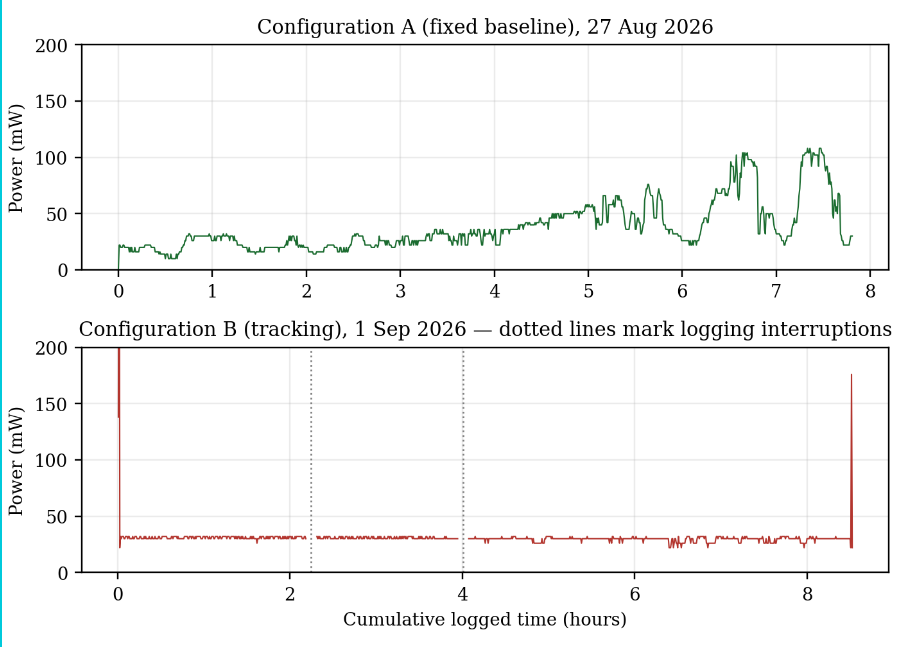
\includegraphics[width=\columnwidth]{figures/fig1_power.png}
\caption{Logged power output over time for both configurations. Configuration B is
shown as its three logged sessions concatenated on a cumulative time axis, with dotted
lines marking the two logging interruptions.}
\label{fig:power}
\end{figure}

\begin{table}[h]
\centering
\caption{Measured Energy and Power Output by Configuration}
\label{tab:energy}
\small
\begin{tabular}{@{}lccc@{}}
\toprule
\textbf{Configuration} & \textbf{Duration (h)} & \textbf{Energy (mWh)} & \textbf{Avg. Power (mW)} \\
\midrule
A (fixed baseline) & 7.81 & 295.68 & 37.87 \\
B, session 1 & 2.18 & 72.08 & 33.02 \\
B, session 2 & 1.64 & 50.11 & 30.52 \\
B, session 3 & 4.46 & 132.60 & 29.74 \\
\midrule
\textbf{B (tracking, total)} & \textbf{8.28} & \textbf{254.79} & \textbf{30.76} \\
\bottomrule
\end{tabular}
\end{table}

The comparison is not valid as a test of tracking. Examination of the logged current
and voltage shows that the two configurations were not operating under equivalent
electrical load, which invalidates any attribution of the measured difference to
tracking or its absence.

Configuration A's current varied across an order of magnitude over the test day,
tracking changes in irradiance as expected of a panel delivering charge to a battery,
and its voltage remained near 4.4V, consistent with a panel clamped to a charging
lithium-polymer cell. Configuration B's current was below 6 mA in 99.7\% of samples and
remained essentially flat and insensitive to conditions, while its voltage sat near
6.3V, above the panel's nominal 5V rating. A panel holding above its nominal voltage
while delivering negligible and irradiance-insensitive current is operating near its
open circuit point, meaning it had no meaningful electrical load drawing power from it.
The most probable causes are that Configuration B's lithium polymer cell had already
reached full charge and its TP4056 module had terminated charging, or that the load
path was not correctly connected for that session.

\begin{figure}[t]
\centering
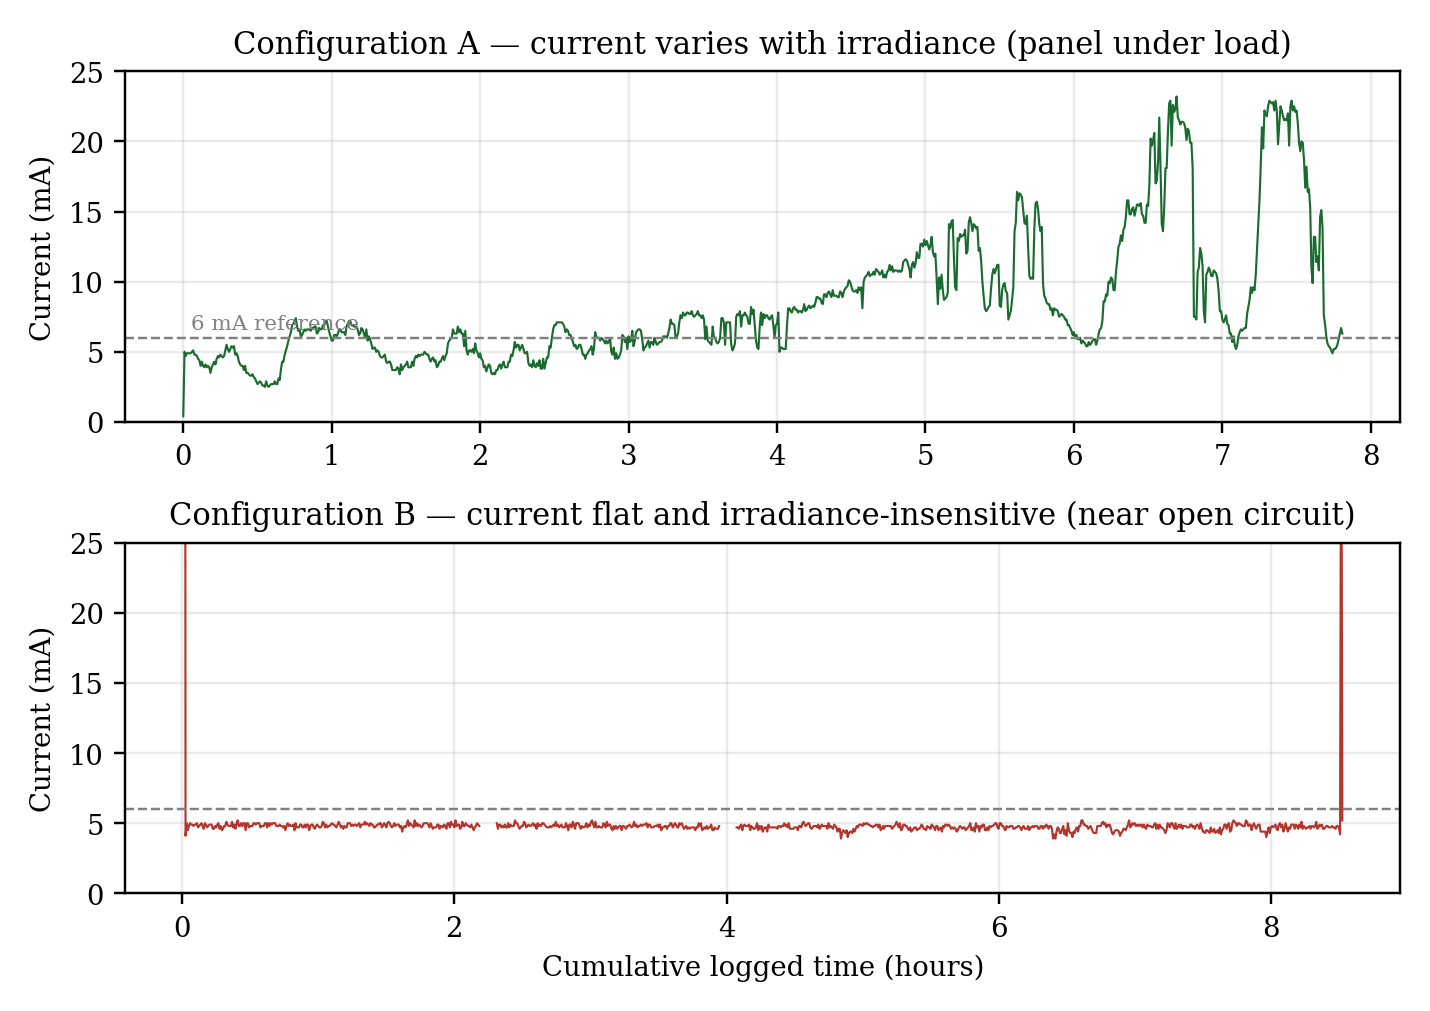
\includegraphics[width=\columnwidth]{figures/fig2_current.png}
\caption{Logged current for both configurations on a common vertical scale.
Configuration A varies across an order of magnitude in response to changing irradiance;
Configuration B remains flat near 5 mA throughout, indicating no meaningful load.}
\label{fig:current}
\end{figure}

\begin{table}[h]
\centering
\caption{Electrical Operating Conditions by Configuration}
\label{tab:electrical}
\small
\begin{tabular}{@{}lcc@{}}
\toprule
\textbf{Quantity} & \textbf{Configuration A} & \textbf{Configuration B} \\
\midrule
Mean current (mA) & 8.47 & 4.94 \\
Current range (mA) & 0.40 -- 23.20 & 3.90 -- 127.90 \\
Samples below 6 mA & 35.5\% & 99.7\% \\
Mean voltage (V) & 4.422 & 6.312 \\
Voltage range (V) & 4.06 -- 4.68 & 4.14 -- 6.62 \\
\bottomrule
\end{tabular}
\end{table}

\begin{figure}[t]
\centering
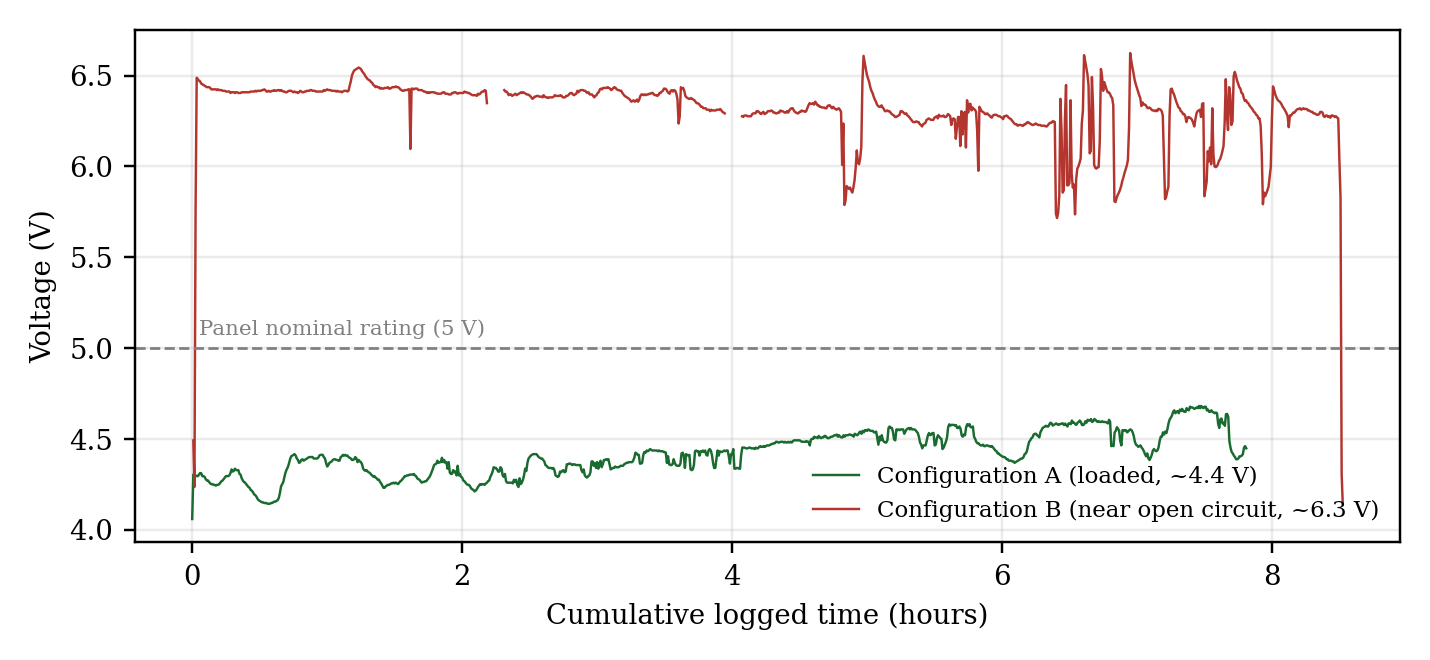
\includegraphics[width=\columnwidth]{figures/fig3_voltage.png}
\caption{Logged voltage for both configurations. Configuration B operates above the
panel nominal rating of 5 V, consistent with open-circuit behaviour, while Configuration
A remains clamped near 4.4 V by the charging cell.}
\label{fig:voltage}
\end{figure}

As power is the product of voltage and current, a panel held near an open circuit
produces low measured power regardless of how well it is aimed. The 18.8\% deficit
therefore reflects unequal load conditions between the two configurations, not an
effect of tracking. Additionally, the two configurations were tested on different days
instead of simultaneously, so day-to-day variation in weather and irradiance is a
further uncontrolled variable. No transformation or normalization of this dataset can
recover a valid tracking comparison from it; a repeat trial with both configurations
under verified equivalent load, logged simultaneously, is required.

\textbf{Tracking behavior.} Independent of the energy comparison, the logged servo
angle and sensor channel permit direct evaluation of the tracking subsystem. The servo
actuated and repositioned the panel over the course of the test, confirming that the
sensor to actuator control path was functional. However, the sensors saturated for much
of each session: both analog channels read the 10-bit ADC ceiling of 1023 simultaneously
in 46\% of all Configuration B samples. When both channels are saturated, the computed
differential is exactly zero, leaving the control loop with no usable directional
signal.

\begin{table}[h]
\centering
\caption{Tracking Behavior by Session}
\label{tab:tracking}
\small
\begin{tabular}{@{}lcccc@{}}
\toprule
\textbf{Session} & \textbf{Dur. (h)} & \textbf{Repos.} & \textbf{Angle range (\textdegree)} & \textbf{Both sat.} \\
\midrule
B, session 1 & 2.18 & 41 & 15--92 & 42\% \\
B, session 2 & 1.64 & 0 & 90 (none) & 99\% \\
B, session 3 & 4.46 & 99 & 30--165 & 28\% \\
\bottomrule
\end{tabular}
\end{table}

\begin{figure}[t]
\centering
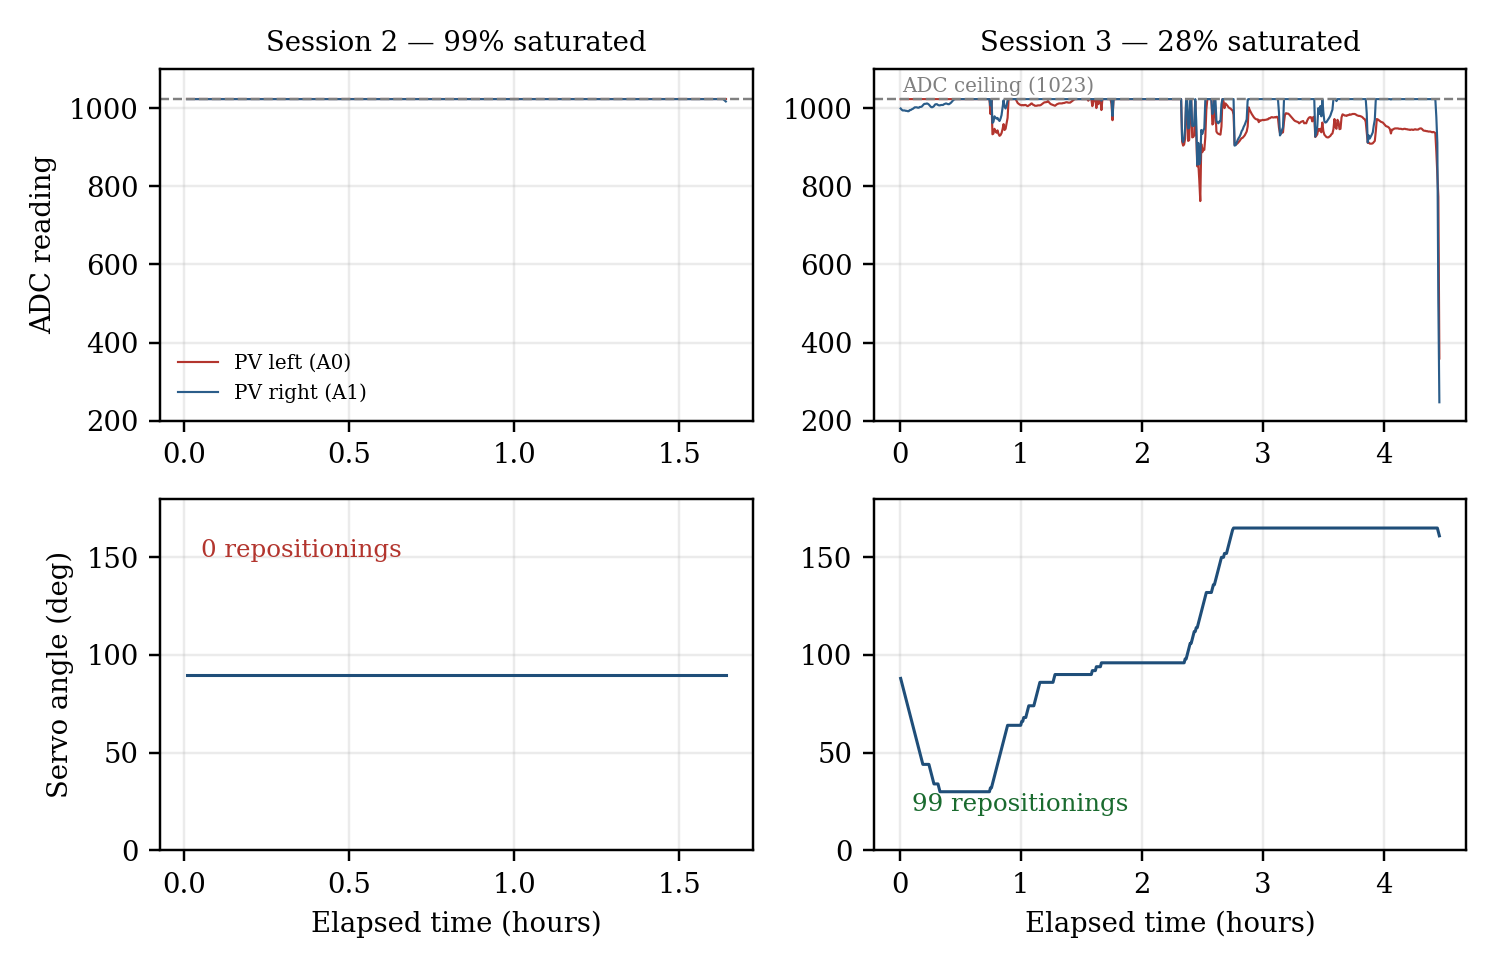
\includegraphics[width=\columnwidth]{figures/fig4_adc_servo.png}
\caption{Sensor readings and corresponding servo response for sessions 2 and 3. With
both channels held at the ADC ceiling throughout session 2, the computed differential
is zero and the panel does not move; in session 3, where the sensors retain usable
range, the control loop repositions the panel 99 times.}
\label{fig:adcservo}
\end{figure}

Session 2 demonstrates the consequence directly: with both sensors saturated in 99\%,
the panel did not get the required signal in order to tilt, causing it to be stuck at
90 degrees for 1 hour 38 minutes. Sessions 1 and 3, with lower rates of saturation,
resulted in 41 and 99 repositionings, respectively. The relationship between sensor
saturation and tracking inactivity is therefore consistent across sessions and
identifies inadequate signal conditioning on the PV sensor channels as the limiting
fault in the tracking subsystem. The PV cells require a series resistor or voltage
divider to bring their full sun-output within the ADC's input range.

In session 3 the panel additionally reached its 165 degree travel limit and remained
there for 1 hour 41 minutes, indicating the commanded angle saturated against the end of
the servo's usable range rather than converging on a tracking position.

\textbf{Tracking Response Time.} The design criterion specified repositioning within
10 minutes of detecting a sufficient differential. Logged intervals between servo
repositionings had a median of 0.5 minutes, with 94 of 98 intervals in sessions 1 and 3
falling under 10 minutes. The implemented control loop therefore satisfies the
response-time criterion, but does so by evaluating and repositioning at the 30-second
logging interval rather than the 10 minute response window described in the design
method. Implemented behavior deviates from the documented specification and the
specification should be corrected to match, or the loop rate reduced as originally
intended to limit servo wear.

\subsection{User Testing}

This project is a data-collection instrument for a controlled physical experiment
rather than a consumer-facing product, so user testing in the conventional sense does
not apply. In its place, this section reports operator-level verification, namely
whether the system can be deployed, started, and its data retrieved and interpreted by
an operator working from this document alone.

Deployment and startup were confirmed, requiring only that both configurations be
positioned outdoors, powered, and left to log. Data retrieval was likewise confirmed,
with logs written in CSV format directly readable in standard spreadsheet software
without preprocessing. Operator verification did, however, identify a significant gap.
The system provides no indication of whether it is logging valid data while a test is
running. The Configuration B load fault reported above was not detectable in the
field and was identified only during post-test analysis, after an entire test day had
been spent collecting data that could not answer the research question. Configuration
B's logging interruptions were likewise invisible to the operator during the run. A
future revision should provide in-field feedback sufficient for an operator to confirm
valid operation before committing a full test day, at minimum an indicator confirming
that measured current exceeds a plausible minimum threshold on both channels.

A second violation of the experimental design compounds this fault. Section IV
specifies simultaneous operation of both configurations under shared ambient
conditions as the mechanism controlling for irradiance and weather variation. The two
configurations were instead tested on separate days, 27 August and 1 September 2026,
leaving inter-day variation in atmospheric conditions uncontrolled. Configuration B's
logging was additionally interrupted twice, yielding three discontinuous records
rather than the single continuous record obtained for Configuration A.

The 10\% energy gain criterion specified in Section II is therefore recorded as not
demonstrated rather than as unmet. No post-hoc normalization or transformation of the
collected data can recover a valid comparison, as the deficiency lies in the
experimental conditions rather than in the treatment of the resulting measurements.

The tracking subsystem, evaluated independently of the energy comparison, yielded
interpretable results. The sensor to actuator control path/loop functioned as
designed, and the panel reacted accordingly. The tracking response criterion was
satisfied with a median interval of 30 seconds.

The limiting fault in the tracking subsystem was the inadequate signal conditioning at
the directional sensor. With the photovoltaic elements connected directly to the
analog input, the channels reached the 10-bit ceiling of 1023 in 46\% of the samples.
The differential used to drive the control was essentially zero, rendering the loop
insensitive. Session 2 provides evidence: with both the channels saturated in 99\% of
samples, no repositioning occurred across 1 hour 38 minutes of operation, while other
sessions with rates of 42\% and 28\% produced 41 and 99 repositioning events,
respectively.

This limitation was anticipated at the design stage. The criterion designated usable
resolution under peak irradiance was included in the sensor decision matrix presented
in Section IV, and the selected option was scored 3 against it. The weight assigned to
that criterion, 0.25, was insufficient to alter the selection outcome, and no
mitigation was incorporated into the implemented design.

\section{Conclusions and Recommendations}

\textbf{Conclusions.} The primary research question, namely the magnitude of the
energy gain attributable to single-axis tracking relative to a fixed baseline, is not
answered by the data collected in this study. Configuration B recorded an average
power output 18.8\% below that of Configuration A, but this result cannot be
interpreted as evidence regarding tracking performance in either direction.

The measured deficit is attributable to unequal electrical loading between the two
configurations rather than to panel orientation. Configuration B operated near its
open-circuit point throughout its test period, drawing less than 6 mA in 99.7\% of
recorded samples while sustaining a bus voltage of approximately 6.3 V, above the 5 W
panel nominal rating of 5 V. A photovoltaic panel exhibiting elevated voltage in
combination with negligible and irradiance-insensitive current is delivering no
appreciable power to a load, and its measured output under such conditions is governed
by the absence of that load rather than by its orientation relative to the sun. The
probable cause is that the lithium-polymer cell associated with Configuration B had
reached full charge, terminating current draw through its TP4056 charge controller, or
alternatively that the load path was not correctly established for the test period.

A second violation of the experimental design compounds this fault. Section IV
describes simultaneous operation of both configurations as the mechanism to account for
irradiance variation. However, both configurations were tested on separate days,
leaving inter-day variation in atmospheric conditions uncontrolled.

The 10\% energy gain criterion specified in Section II is therefore recorded as not
demonstrated rather than as unmet. No post-hoc normalization or transformation of the
collected data can recover a valid comparison, as the deficiency lies in the
experimental conditions rather than in the treatment of the resulting measurements.

\textbf{Recommendations.}

\begin{itemize}
\item \textbf{Incorporate signal conditioning at the directional sensor inputs.} A
series divider should be created such that the PV sensor output under peak irradiance
corresponds to $\sim$80\% of the analog-to-digital converter input range, allowing the
differential resolution to be preserved.
\item \textbf{Verify load condition prior to each test period.} Both lithium-polymer
cells should be discharged to a partial state, such that their respective charge
controllers draw current throughout the test window.
\item \textbf{Instrument the system for in-field validation confirmation.} The system
as constructed provides no indication of measurement validity during operation. The
Configuration B loading fault was identified only during post analysis, after a
complete period had elapsed.
\item \textbf{Repeat the comparison under simultaneous logged operation.} Simultaneous
operation was specified in the design method but not achieved in execution, and
represents the single modification most consequential to the validity of the result.
\item \textbf{Extend the measurement to net energy gain.} Servo current draw was not
separately accounted for in the energy comparison. Subsequent work should measure
actuator consumption independently, and report tracking gain of the energy expended in
achieving it.
\end{itemize}

\textbf{Concluding Remark.} The outcome of this study illustrates a distinction
relevant to instrumented experimental work generally: a system that operates without
interruption and produces well-formed output is not thereby producing valid data.
Configuration B logged continuously for in excess of eight hours and returned
correctly structured records throughout, and the fault was detectable only by
evaluating whether the logged current was physically consistent with the expected
behavior of a loaded photovoltaic panel. Verification that measured quantities are
physically plausible, rather than confirmation that measurement occurred, is the
practice most clearly demonstrates the necessity of.

\begin{thebibliography}{9}

\bibitem{awasthi2020}
A. Awasthi, A. K. Shukla, M. M. Srivastava, C. Dondariya, K. N. Shukla, D. Porwal, and
G. Richhariya, ``Review on sun tracking technology in solar PV systems,'' \emph{Energy
Reports}, vol. 6, pp. 392--405, 2020.

\bibitem{guiza2019}
D. Guiza, D. Ounnas, Y. Soufi, and M. Maamri, ``Implementation of perturb and observe
based MPPT algorithm for photovoltaic systems,'' 2019.

\bibitem{jamroen2021}
C. Jamroen, C. Fongkerd, W. Krongpha, P. Komkum, A. Pirayawaraporn, and N.
Chindakham, ``A novel UV sensor-based dual-axis solar tracking system: Implementation
and performance analysis,'' \emph{Applied Energy}, vol. 299, Art. 117295, 2021.

\bibitem{killi2015}
M. Killi and S. Samanta, ``Modified perturb and observe MPPT algorithm for drift
avoidance in photovoltaic systems,'' \emph{IEEE Transactions on Industrial
Electronics}, vol. 62, no. 9, pp. 5549--5559, 2015.

\bibitem{okwu2025}
M. O. Okwu, O. P. Eruero, N. Abubakar, B. A. Edward, B. U. Oreko, O. B. Otanocha, O.
F. Orikpete, C. Maware, K. C. Ezekiel, C. Ori, and L. Tartibu, ``Single-axis solar
tracking systems: A comprehensive design and performance study,'' \emph{Procedia
Computer Science}, 2025.

\bibitem{oumarou2015}
M. B. Oumarou, A. A. Toyin, and F. A. Oluwole, ``Design optimization and performance
evaluation of a single axis solar tracker,'' \emph{Sustainable Energy}, vol. 3, no. 1,
pp. 9--13, 2015.

\bibitem{tanduri2025}
G. Tanduri, ``Single axis automatic solar tracking system,'' \emph{International
Journal of Research and Scientific Innovation}, vol. 12, no. 7, pp. 2188--2192, 2025.

\bibitem{wang2013}
J.-M. Wang and C.-L. Lu, ``Design and implementation of a sun tracker with a dual-axis
single motor for an optical sensor-based photovoltaic system,'' \emph{Sensors}, vol.
13, no. 3, pp. 3157--3168, 2013.

\end{thebibliography}

\appendices

\section{Hardware (CAD layout, circuit layout)}

\begin{figure}[h]
\centering
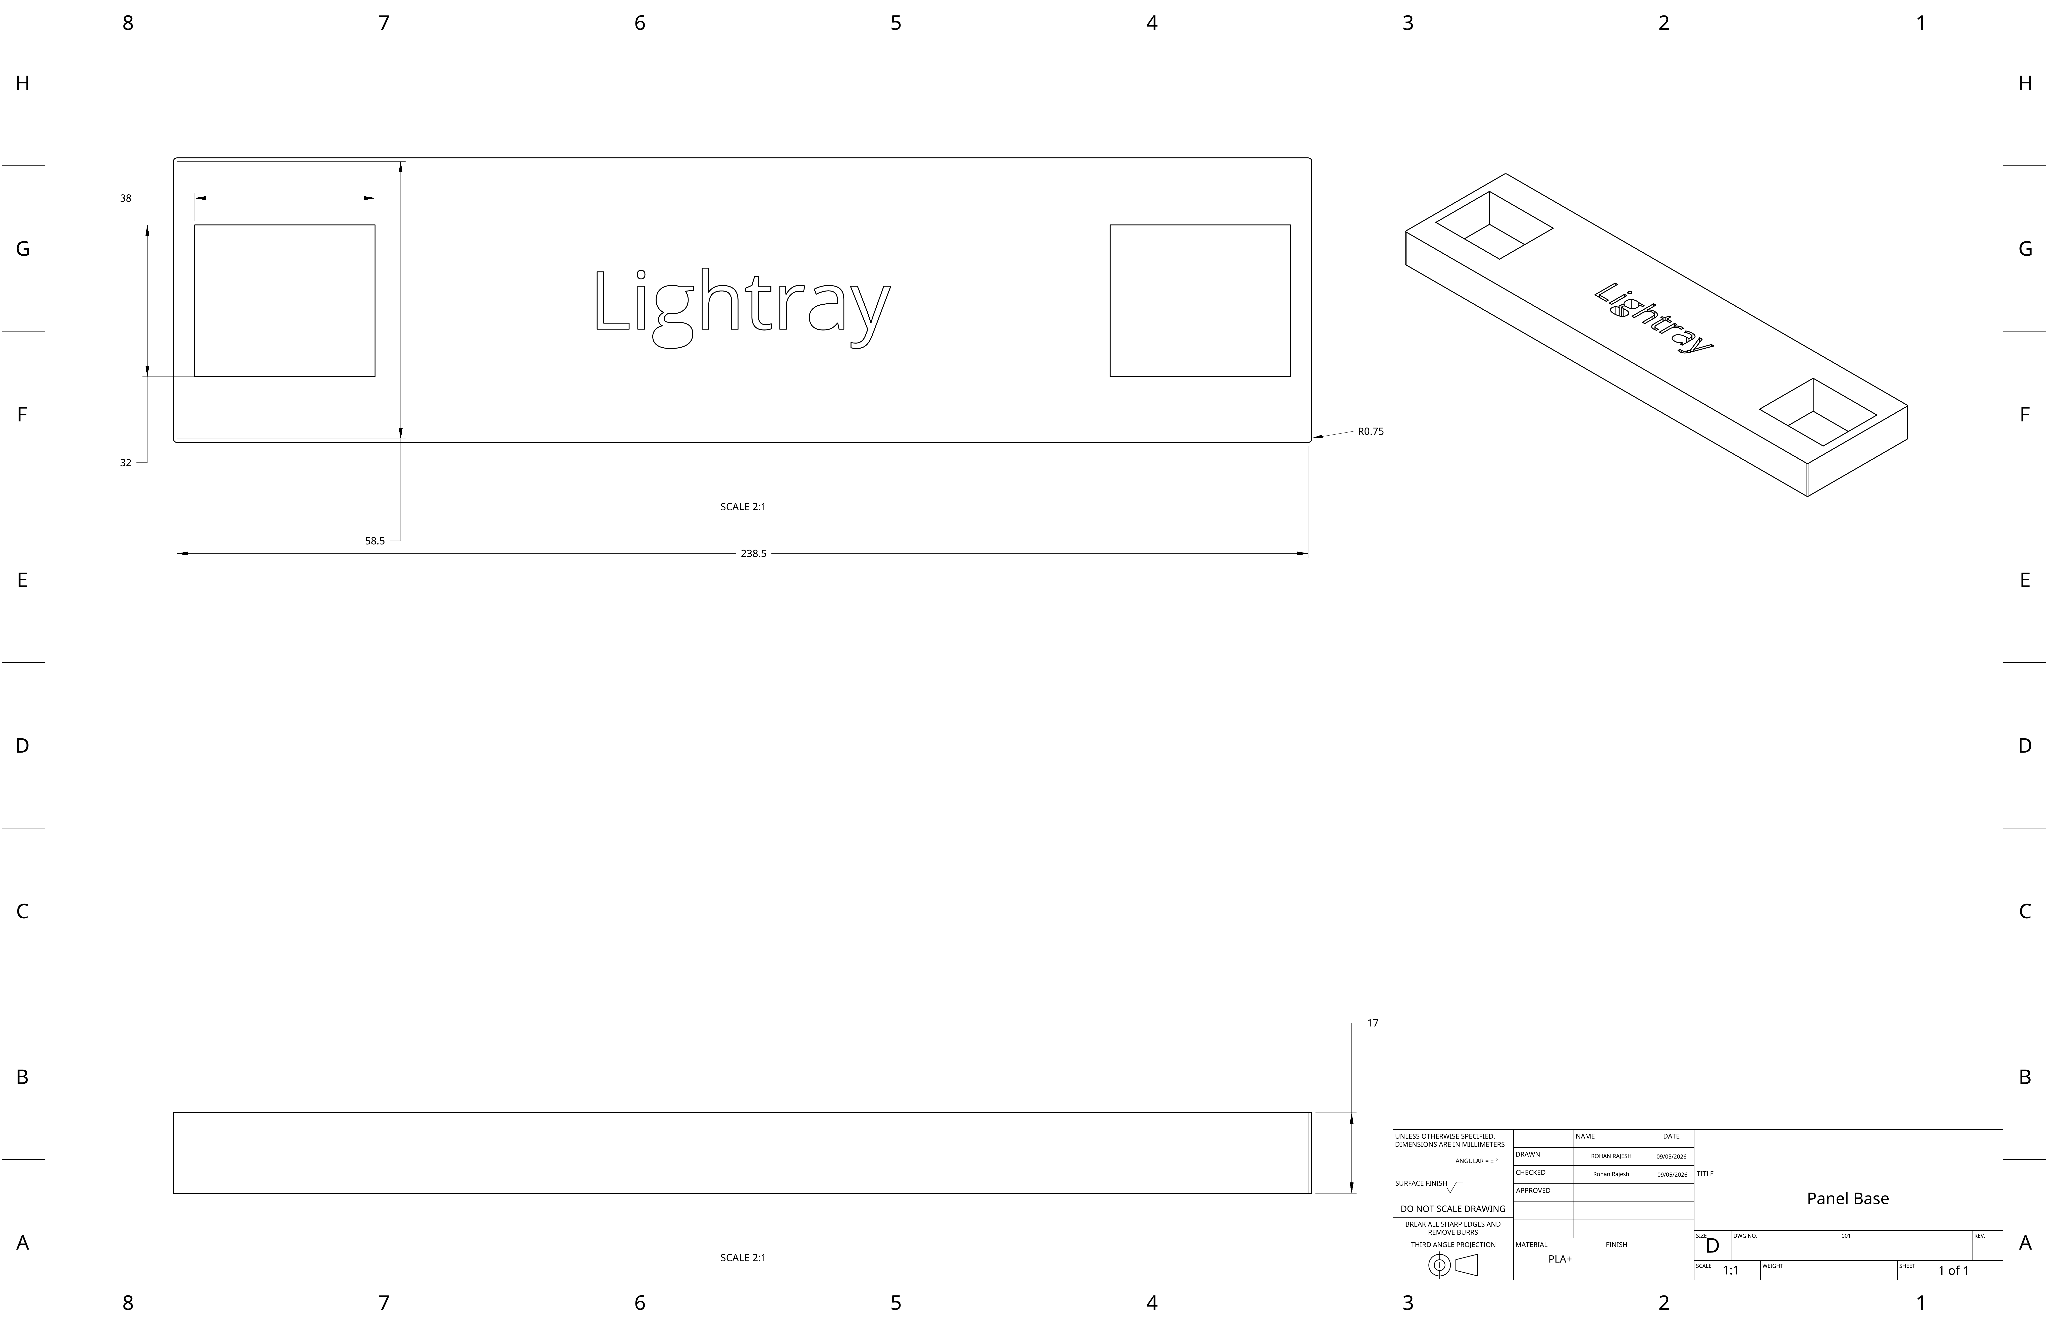
\includegraphics[width=\columnwidth]{figures/cad_panel_base.png}
\caption{Panel base CAD drawing.}
\end{figure}

\begin{figure}[h]
\centering
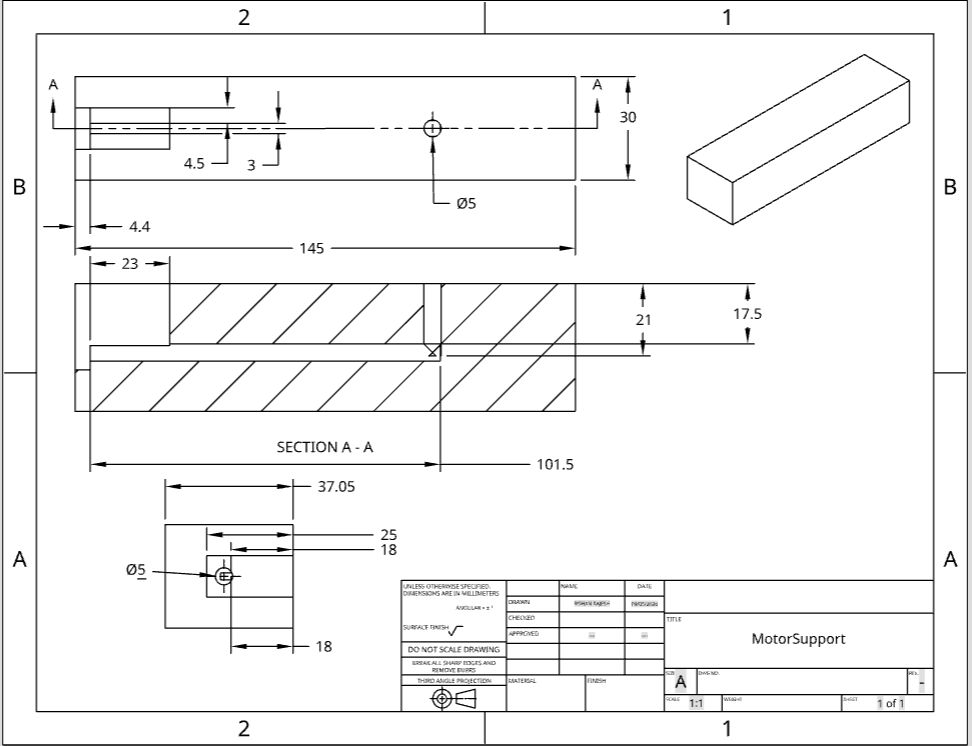
\includegraphics[width=\columnwidth]{figures/cad_motor_support.png}
\caption{Motor support/motor bar CAD drawing.}
\end{figure}

\begin{figure}[h]
\centering
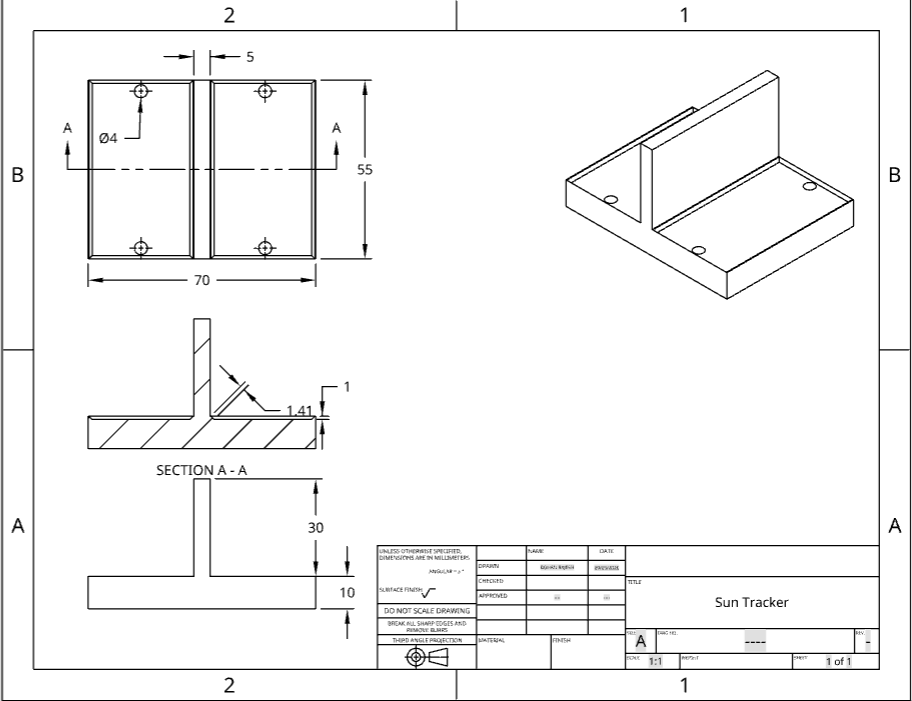
\includegraphics[width=\columnwidth]{figures/cad_sun_tracker.png}
\caption{Sun tracker bracket CAD drawing.}
\end{figure}

\begin{figure}[h]
\centering
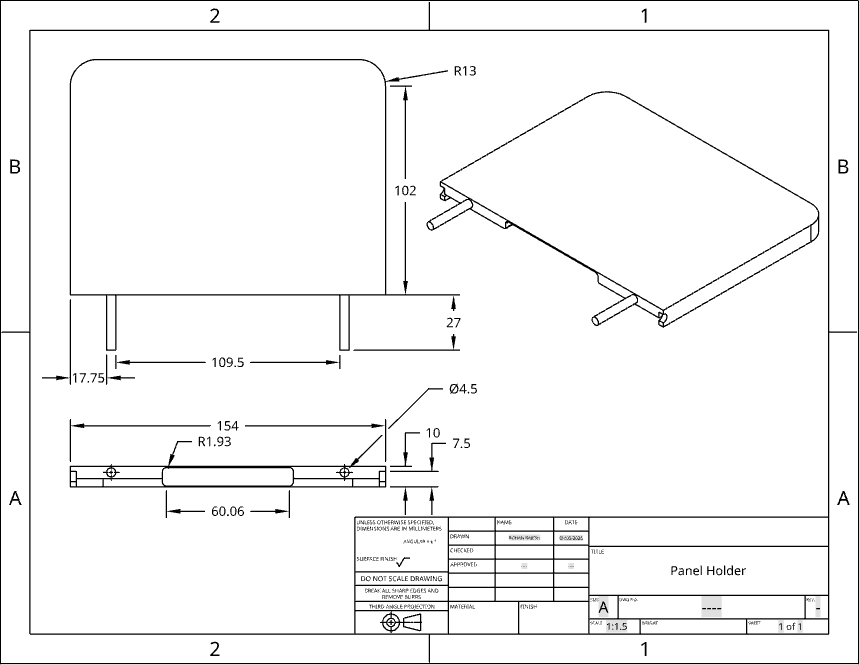
\includegraphics[width=\columnwidth]{figures/cad_panel_holder.png}
\caption{Panel holder CAD drawing.}
\end{figure}

\begin{figure}[h]
\centering
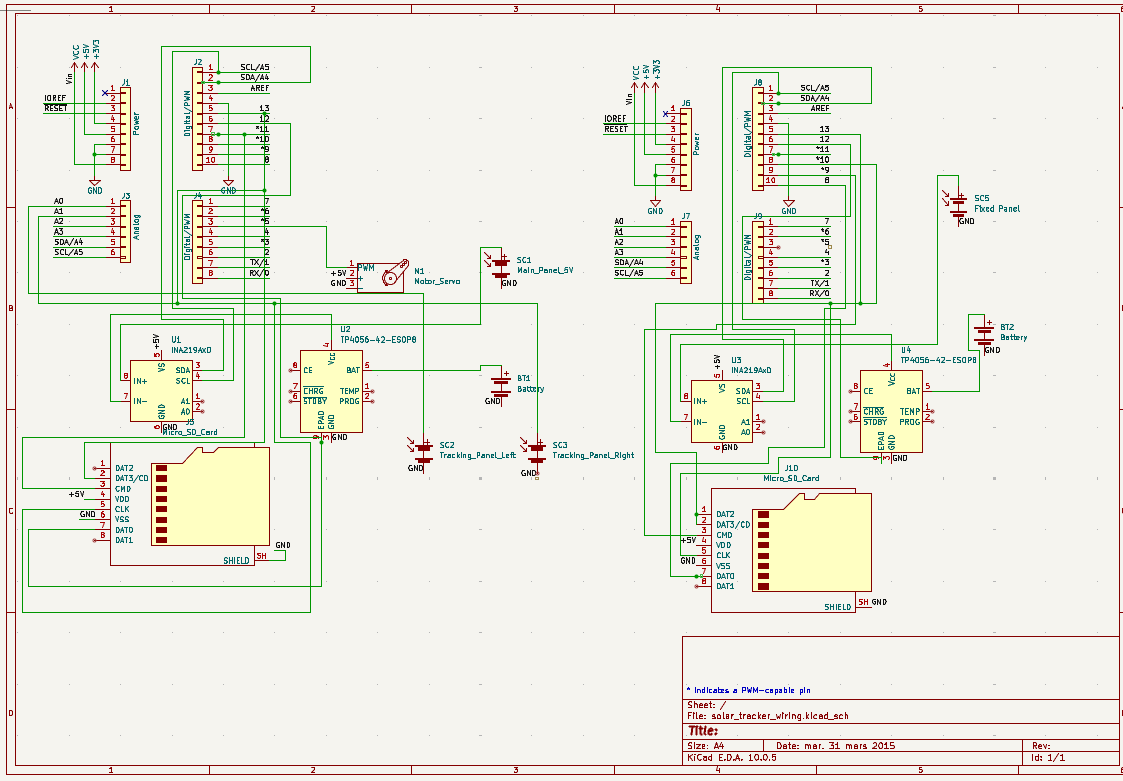
\includegraphics[width=\columnwidth]{figures/schematic.png}
\caption{KiCad wiring schematic for both configurations.}
\end{figure}

\section{Software (pseudocode, code)}

\subsection{Pseudocode}

\begin{lstlisting}
CONSTANTS
  SAMPLE_INTERVAL = 30000 ms      // logging and control period
  DIFF_THRESHOLD  = 15            // ADC counts; below this, treat as noise
  STEP_SIZE       = 2             // degrees per correction
  ANGLE_MIN       = 15            // servo travel limits
  ANGLE_MAX       = 165
  START_ANGLE     = 90            // centred at power-on
  SUPPORT_ANGLE   = 90            // passive support servo (D6)

PINS
  A0 -> pv_left     analog input, PV sensor, left of divider
  A1 -> pv_right    analog input, PV sensor, right of divider
  D9 -> tracking servo   PWM output
  D6 -> support servo    PWM output, detached after centring
  SDA/SCL -> INA219      I2C, power monitoring
  ICSP -> SD card        hardware SPI

SETUP
  initialise serial, I2C, SD card
  IF SD card fails to initialise THEN halt and signal error
  write CSV header row to log file

  attach support servo on D6
  command support servo to SUPPORT_ANGLE
  wait until movement to complete
  detach support servo     // becomes a passive pivot, not an actuator

  attach tracking servo on D9
  set current_angle = START_ANGLE
  command tracking servo to current_angle

  initialise INA219
  IF INA219 not detected THEN halt and signal error

  record start time

MAIN LOOP (executed once per SAMPLE_INTERVAL)
  // ---- read directional sensors ----
  pv_left  = analogRead(A0)
  pv_right = analogRead(A1)
  differential = pv_right - pv_left

  // ---- tracking decision ----
  IF absolute_value(differential) > DIFF_THRESHOLD THEN
    IF differential > 0 THEN            // right cell brighter
        target_angle = current_angle + STEP_SIZE
    ELSE                                 // left cell brighter
        target_angle = current_angle - STEP_SIZE
    END IF
    constrain target_angle between ANGLE_MIN and ANGLE_MAX
    IF target_angle != current_angle THEN
        command tracking servo to target_angle
        current_angle = target_angle
    END IF
  END IF
  // no correction is applied when the differential is within threshold,
  // which includes the case where both channels are saturated at 1023
  // and the differential is therefore identically zero

  // ---- power measurement ----
  bus_voltage = INA219.getBusVoltage_V()
  current_mA  = INA219.getCurrent_mA()
  power_mW    = INA219.getPower_mW()

  // ---- logging ----
  elapsed = millis() - start_time
  open log file
  write row: elapsed, formatted_time, pv_left, pv_right,
             current_angle, bus_voltage, current_mA, power_mW
  close log file

  wait until SAMPLE_INTERVAL has elapsed since last iteration
END LOOP
\end{lstlisting}

\subsection{Final Code}

\begin{lstlisting}
/*
 Config B -- Single-Axis Solar Tracker
 Pioneer Academics Research Project (Rohan Rajesh)

 Reads two PV sensor cells (A0/A1) as directional light sensors,
 steps two servos (D9, D6) to point the panel at the brighter side, and
 logs PV readings + INA219 power data to SD for the daily energy
 comparison against the fixed baseline (Config A). Servo 2 mirrors
 servo 1's angle by default.
*/
#include <Wire.h>
#include <Adafruit_INA219.h>
#include <Servo.h>
#include <SPI.h>
#include <SD.h>

// ---- Pin assignments ----
const int PV_LEFT_PIN  = A0;
const int PV_RIGHT_PIN = A1;
const int SERVO_PIN    = 9;
const int SERVO2_PIN   = 6;   // second servo, mirrors tracking angle by default
const int SD_CS_PIN    = 10;

// ---- Tracking parameters ----
const int SERVO_MIN_ANGLE = 15;
const int SERVO_MAX_ANGLE = 165;
const int SERVO_STEP      = 2;      // degrees moved per correction
const int DEADBAND        = 15;     // raw ADC diff, ignores sensor noise
const unsigned long CHECK_INTERVAL = 30000UL; // 1 min, well under the 10 min spec

// ---- Globals ----
Servo trackerServo;
Servo trackerServo2;
Adafruit_INA219 ina219;
int currentAngle = 90;
unsigned long lastCheck = 0;
bool sdReady = false;

void setup() {
  Serial.begin(9600);

  trackerServo.attach(SERVO_PIN);
  trackerServo.write(currentAngle);   // start centered

  trackerServo2.attach(SERVO2_PIN);
  trackerServo2.write(currentAngle);  // center it once
  delay(300);                         // give it time to actually reach
                                       // center before releasing
  trackerServo2.detach();             // no more pulses = no holding torque,
                                       // free to be pushed by the panel

  Wire.begin();
  if (!ina219.begin()) {
    Serial.println(F("INA219 not found. Check wiring/I2C address."));
  }

  if (!SD.begin(SD_CS_PIN)) {
    // don't halt the whole tracker just because logging failed
    Serial.println(F("SD init failed. Logging disabled, tracking still runs."));
    sdReady = false;
  } else {
    sdReady = true;
    File logFile = SD.open("track.csv", FILE_WRITE);
    if (logFile) {
      logFile.println(F("millis,pv_left,pv_right,angle,bus_v,current_mA,power_mW"));
      // CSV header, written once
      logFile.close();
    }
  }
}

void loop() {
  unsigned long now = millis();
  if (now - lastCheck < CHECK_INTERVAL) return; // skip until next check window
  lastCheck = now;

  int pvLeft  = averageRead(PV_LEFT_PIN);
  int pvRight = averageRead(PV_RIGHT_PIN);
  int diff = pvLeft - pvRight;

  if (abs(diff) > DEADBAND) {
    currentAngle += (diff > 0) ? -SERVO_STEP : SERVO_STEP;
    // move toward brighter side
    currentAngle = constrain(currentAngle, SERVO_MIN_ANGLE, SERVO_MAX_ANGLE);
    // keep servo off its stops
    trackerServo.write(currentAngle);
    // trackerServo2 is detached, it's a free pivot now, gets pushed
    // along by the panel
  }

  // pull power data for this same check window, logged alongside
  // tracking state
  float busVoltage = ina219.getBusVoltage_V();
  float current_mA = ina219.getCurrent_mA();
  float power_mW   = ina219.getPower_mW();

  if (sdReady) {
    logData(pvLeft, pvRight, currentAngle, busVoltage, current_mA, power_mW);
  }

  Serial.print(F("L:")); Serial.print(pvLeft);
  Serial.print(F(" R:")); Serial.print(pvRight);
  Serial.print(F(" angle:")); Serial.print(currentAngle);
  Serial.print(F(" V:")); Serial.print(busVoltage);
  Serial.print(F(" mA:")); Serial.println(current_mA);
}

// 10-sample average, kills single-read ADC noise
int averageRead(int pin) {
  long sum = 0;
  const int samples = 10;
  for (int i = 0; i < samples; i++) {
    sum += analogRead(pin);
    delay(5);
  }
  return sum / samples;
}

// appends one CSV row, opens/closes each call so a crash doesn't
// corrupt the file
void logData(int pvL, int pvR, int angle, float v, float mA, float mW) {
  File logFile = SD.open("track.csv", FILE_WRITE);
  if (logFile) {
    logFile.print(millis()); logFile.print(",");
    logFile.print(pvL); logFile.print(",");
    logFile.print(pvR); logFile.print(",");
    logFile.print(angle); logFile.print(",");
    logFile.print(v); logFile.print(",");
    logFile.print(mA); logFile.print(",");
    logFile.println(mW);
    logFile.close();
  }
}
\end{lstlisting}

\section{Images and Videos}

\begin{figure}[h]
\centering
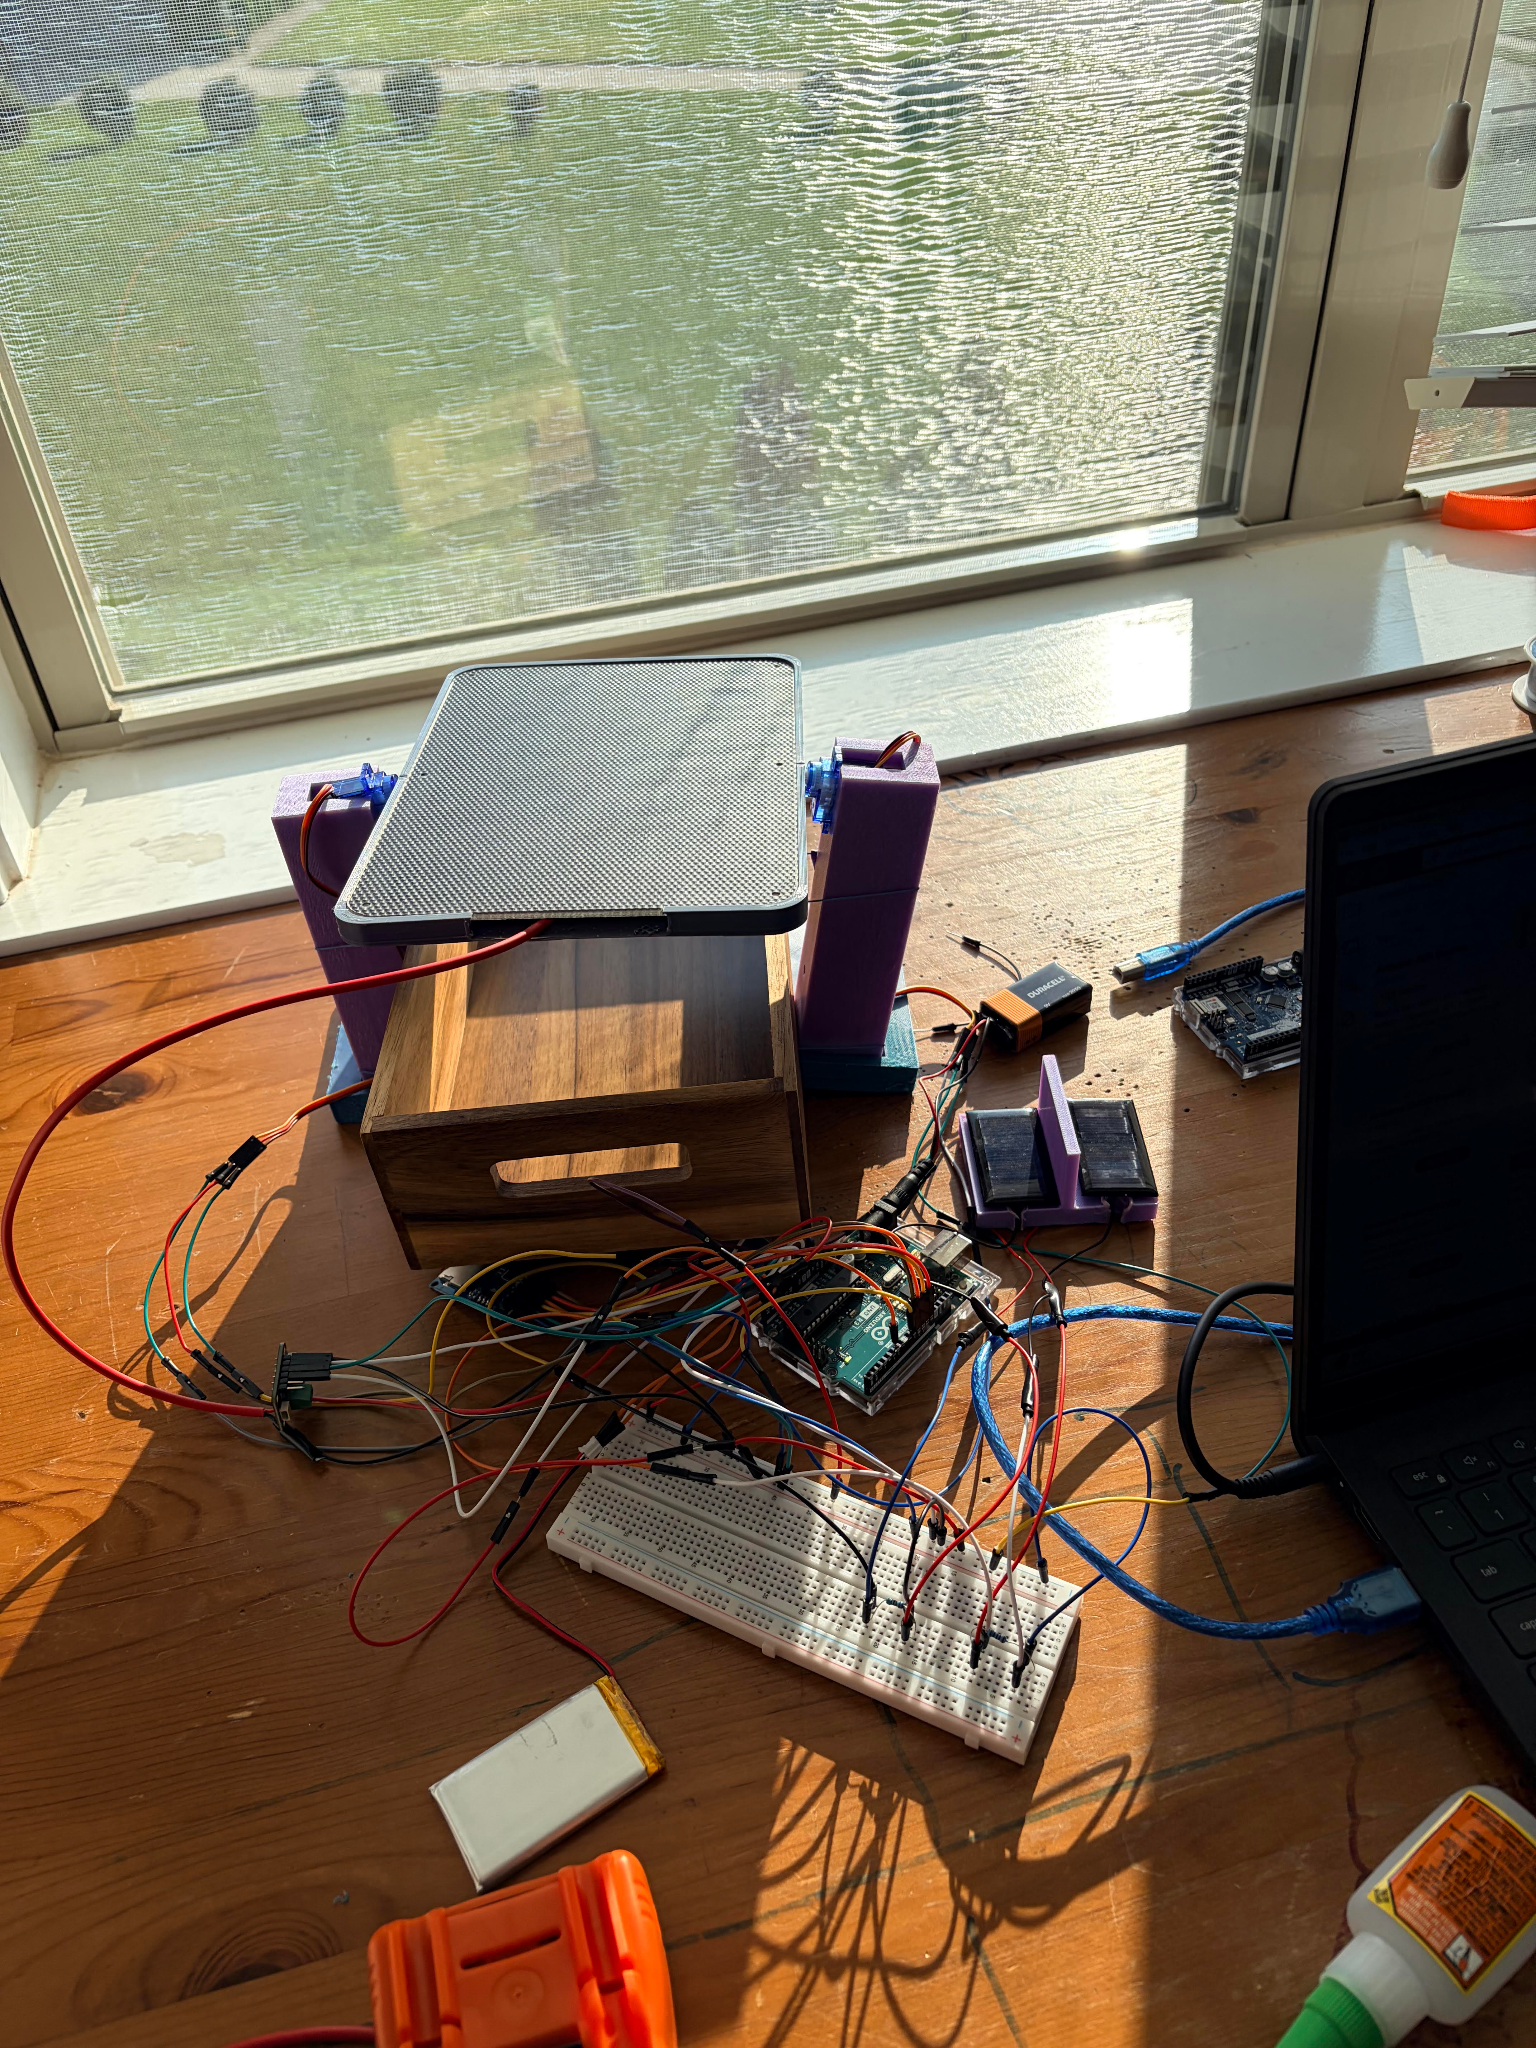
\includegraphics[width=0.7\columnwidth]{figures/prototype_photo.png}
\caption{Physical prototype: Arduino Uno, breadboard, INA219 modules, servo-driven
tracking bracket, and fixed baseline stand.}
\end{figure}

\end{document}
